%!TEX root = talk612.tex

%!TEX root = thesis.tex

\documentclass[a4paper]{article}
\usepackage{amsthm}
\usepackage[utf8]{inputenc}
\usepackage{csquotes}
\usepackage[english]{babel}
\usepackage{graphicx}
\usepackage{enumitem}
\usepackage{subcaption}  %ALLOWS SUBFIGURES
\usepackage{wrapfig}

\usepackage[draft]{fixme}
\fxsetup{theme = color}
\definecolor{fxnote}{rgb}{0.0000, 0.6000,0.0000}
\definecolor{fxwarning}{rgb}{1.0000,0.5490,0.0000}
\definecolor{fxerror}{rgb}{1.0000,0.2706,0.0000}
\definecolor{fxfatal}{rgb}{1.0000,0.0000,0.0000}
\usepackage[backend=biber, giveninits =true, isbn=false, url=false, maxbibnames=100]{biblatex}
\usepackage{hyperref}

%Theorems
\newtheorem{thrm}{Theorem}
\newtheorem{lemma}[thrm]{Lemma}
\newtheorem{prop}[thrm]{Proposition}
\newtheorem{remark}[thrm]{Remark}

\theoremstyle{definition}
\newtheorem*{defi}{Definition}

%%BeginIpePreamble
\usepackage{amsmath}
\usepackage{amssymb}
\usepackage{amsopn}

\newcommand{\scr}[1]{\mathcal{#1}}
\newcommand{\Z}{\mathbb{Z}}
\newcommand{\F}{\mathbb{F}}
\newcommand{\R}{\mathbb{R}}
\newcommand{\N}{\mathbb{N}}
\newcommand{\Q}{\mathbb{Q}}


%Operators
\newcommand{\id}{\operatorname{Id}}



%braces etc
\newcommand{\braces}[1]{\left\lbrace {#1} \right\rbrace}
\newcommand{\sqbr}[1]{\left\lbrack {#1} \right\rbrack }
\newcommand{\abs}[1]{\left\lvert {#1} \right\rvert }
\newcommand{\ceil}[1]{\left\lceil{ #1 } \right\rceil}
\newcommand{\floor}[1]{\left \lfloor {#1}\right\rfloor}
\newcommand{\parens}[1]{\left( {#1} \right)}


%utility
\newcommand{\inv}[1]{{#1}^{-1}}
\newcommand{\half}{\frac{1}{2}}
\newcommand{\third}{\frac{1}{3}}
\newcommand{\goes}{\rightarrow}
\newcommand{\nin}{\not \in}
\newcommand{\sm}[1]{\setminus \braces{#1} }

%vectors and matrices
\newcommand{\zerov}{\vec{0}}
\newcommand{\onev}{\vec{1}}

\newcommand{\twovec}[2]{\parens{ \begin{array}{c}#1 \\ #2\end{array} }}
\newcommand{\threevec}[3]{\prens{ \begin{array}{c}#1 \\ #2\\#3 \end{array} }}
\newcommand{\fourvec}[4]{\parens{ \begin{arr\newcommand{\ifftext}{if and only if }ay}{c}#1 \\ #2\\#3\\#4 \end{array} }}
\newcommand{\twomatrix}[4]{\parens{\begin{array}{cc}#1 & #2 \\ #3 & #4 \end{array}  }}
\newcommand{\twodiagmatrix}[2]{\parens{\begin{array}{cc}#1 & 0 \\ 0 & #2 \end{array}  }}

%%%%THIS THESIS
\newcommand{\intplus}{\operatorname{Int^{+}}}
\newcommand{\interior}{\operatorname{Int}}
\newcommand{\spl}{\operatorname{split}}
\newcommand{\mrg}{\operatorname{merge}}


\newcommand{\ext}[1]{\bar{#1}}
\newcommand{\tightext}[1]{\bar{#1}_t}
\newcommand{\dualgraph}[1]{\G(#1)}
\newcommand{\extdualgraph}[1]{\G_{\scr E}(#1)}



\newcommand{\W}{\scr W}
\renewcommand{\P}{\scr P}
\newcommand{\C}{\scr C}
\newcommand\restrict[1]{\raisebox{-.5ex}{$|$}_{#1}}
\newcommand{\restC}[1]{\ensuremath{\C\restrict{#1}}}

%p is for pole
\newcommand{\pN}{\mathrm{N}}
\newcommand{\pS}{\mathrm{S}}
\newcommand{\pE}{\mathrm{E}}
\newcommand{\pW}{\mathrm{W}}

\newcommand{\cpath}{\C \setminus \braces{\pS}} %cycle path

\newcommand{\rel}{\text{regular edge labeling }}

%%EndIpePreamble


%bib stuff
\bibstyle{plain}

\addbibresource{../thesis.bib}


\title{Investigations}
\author{Sander Beekhuis}
\date{\today} %\today%


\begin{document}
\maketitle

\subsection*{Form all cornerassignments without any seperating $4$-cycle a onesided dual. }
False

Then it also follows that there are no onesided colorings of this graph.



\subsection*{Any valid exteneded graph is a 5-connected traingulation minus one edge.}


\begin{lemma}
  \label{lm:5connIsNoSep4C}
  For plane triangulations having no separating 4-cycle is the same as being 5-connected
\end{lemma}

\begin{proof}
We will show this by contraposition (i.e. having a separating 4-cycle is equivalent to not being 5-conencted).
If a traingulation $G$ has a separating 4-cyle then the nodes of this $4$-cycle are a $4$-cutset and $G$ is not $5$-connected.
On the other hand, if a triangulation is not $5$ connected there is a cutset $X$ of size at most $4$. Removing $X$ splits $G$ into several connected components. By the property that $G$ maximally planar the nodes in $X$ must form a cycle. (They should form a closed curve preventing edges from the one component to the other one.)
\end{proof}

\subsection*{When we remove an edge from a 5-connected triangulation we get a valid extended graph without any seperating 4-cycle.}

\begin{proof}
  Let $G$ be any 5 connected plane triangulation. By Lemma \ref{lm:5connIsNoSep4C} we know that $G$ has no separating $4$-cycle. If we consider any edge $e$ and $\tilde{G} = G \setminus{e}$ then certainly $\tilde{G}$ also has no seperting $4$-cycle. Since any separting $4$-cycle of $\tilde{G}$ would have already been one of $G$.
\end{proof}

Note that a $5$-conneted graph minus one edge is not necessarily again $5$-connected.

Unfortunatly not all extended graphs without seperating $4$-cyles can be generated this way. Conside for example the graph in Figure \ref{fig:ure}. This example has been checked by hand and python on not containing 4cycles.

\begin{figure}[h]
  \centering
  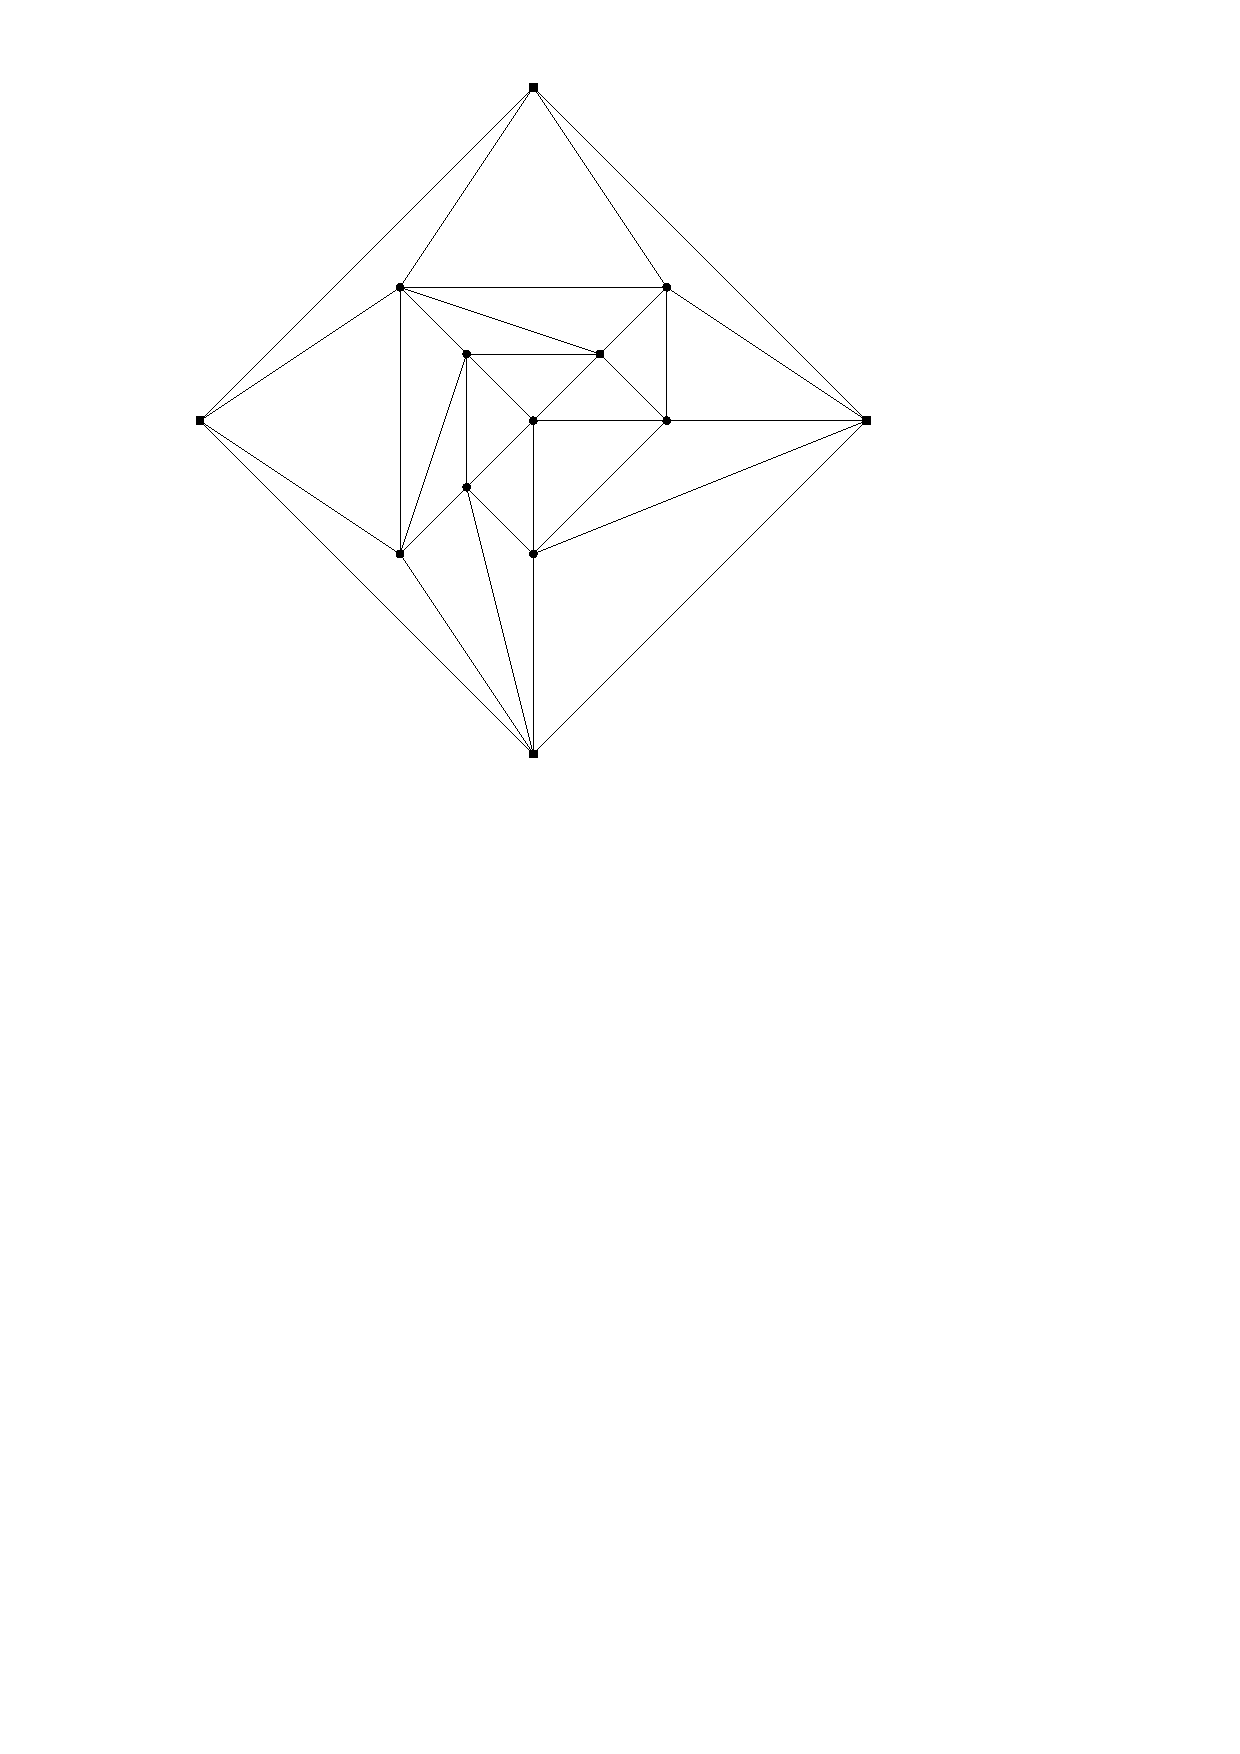
\includegraphics[scale=1]{NoSeperating4CycleButAdddingEdgeBackInIsBad.pdf}
  \caption{}
  \label{fig:ure}
\end{figure}

\section{5-connected traingulations}
5 connected triangulations can be created iteratively using a number of moves.



\section{Failed attempts}
I tried to build a 5-conencted triangulation REL using the limited amount of moves we can do to create other 5-conenected triangulations. I did also view this in the dual.

Unfortunately there are valid REL's with valid moves that we can't color.

\paragraph{Planar seproatrs}
I tried something using planar separators. Unfortunately both sides seem to depend to much upon each other.

\paragraph{Dual}
I currently look at the dual. It seems slightly easier.

\paragraph{Building a REL}
We can build a REL using the steps of constructing a 5-connected triangulation. Unfortunatly it is a bad one.
Base graph and lots of step 3.


\paragraph{}
There is omly one graph with faces of degree 5 and nothing else


\section{Conjectures}
All valid extended graphs can be generated from a base graph and a set of moves. Similarly to 5 connected triangulations.

This rpoblem might be FTP in high degree nodes or NP-haard


\section{Other ideas}
Maybe we can uses Birkenhoff and find sets that are flipped a certain number of times

Some combined red/blue step

A planar separator going trough faces of a low degree (can be large, but this are relivly horles faces if an edge flip goes trough them).

Inside the separator we must have no crossing paths. (This might be restrictive on colorings inf the inside is just a path.)

Planar separator on primal?


Build a REL using consttuction steps. If it goes wrong, reverse change color and try again.

Can we always finish a valid partial coloring? (Of dual and or primal)


Induction on construction steps?
%\listoffixmes

\section{TODO}
Completly read paper. Snap daarna miisscien hoe je zo'n graaf goed opdeeld


\printbibliography
\end{document}
